\documentclass[a4paper, 12pt]{article}
\usepackage{graphicx}
\usepackage[none]{hyphenat}
\usepackage{listings}
\usepackage[english]{babel}
\usepackage{caption}
\usepackage{hyperref}
\usepackage{booktabs}
\usepackage{array}
\usepackage{amsmath}
\usepackage{amssymb}
\usepackage{xcolor}
\usepackage{wrapfig}
\usepackage{fancyhdr}
\usepackage[a4paper, margin=1in]{geometry}

\maxdeadcycles=200
\extrafloats{100}

\lstset{
  frame=single,
  breaklines=true
}

\newcommand{\mydet}[1]{\ensuremath{\begin{vmatrix}#1\end{vmatrix}}}
\providecommand{\brak}[1]{\ensuremath{\left(#1\right)}}
\providecommand{\norm}[1]{\left\lVert#1\right\rVert}
\newcommand{\solution}{\noindent \textbf{Solution: }}
\newcommand{\myvec}[1]{\ensuremath{\begin{pmatrix}#1\end{pmatrix}}}
\let\vec\mathbf

\begin{document}

\begin{center}
    \textbf{\textcolor{blue}{\large CHAPTER-5}} \\
    \vspace{20pt}
    \textbf{\textcolor{blue}{\huge CONTINUITY}}
     \vspace{8pt}
    \textbf{\textcolor{blue}{\huge AND}}
    \vspace{8pt}
    \textbf{\textcolor{blue}{\huge DIFFERENTIABILITY}}
\end{center}

\begin{center}
    \begin{quote}
        \textit{\textcolor{blue}{\large "The whole of science is nothing more than a refinement of everyday thinking."}} \\
        \begin{flushright}
            \textbf{– ALBERT EINSTEIN}
        \end{flushright}
    \end{quote}
\end{center}

\pagestyle{fancy}
\fancyhf{} % Clear default settings
\fancyhead[L]{MATHEMATICS} % Left header
\fancyhead[C]{} % Center header (empty)
\fancyhead[R]{\thepage} % Right header (Page number)
\fancyfoot[C]{2019-20} % Centered footer text
\renewcommand{\headrulewidth}{0pt} % Remove header line
\renewcommand{\footrulewidth}{0pt} % Remove footer line

\vspace{10pt}
\textbf{\textcolor{blue}{\large 5.1 Introduction}}
\vspace{15pt}

\begin{wrapfigure}{r}{0.2\textwidth}
\centering
\vspace{-1cm}
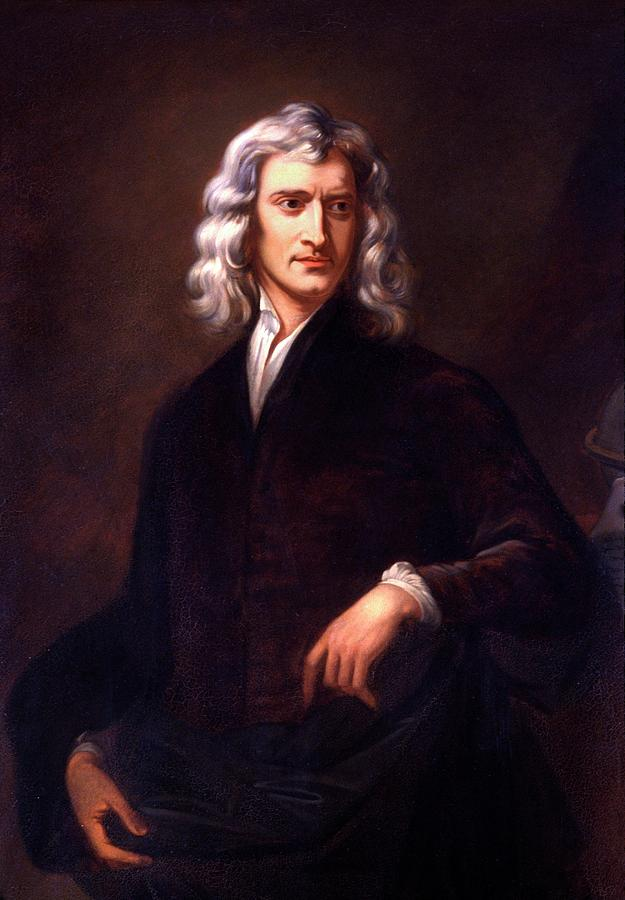
\includegraphics[ width=1\linewidth]{newton.jpg} 
\caption\textbf{Sir Isaac Newton (1642-1727)}
\end{wrapfigure}

This chapter is essentially a continuation of our study of differentiation of functions in Class XI. We had learnt to differentiate certain functions like polynomial functions and trigonometric functions. In this chapter, we introduce the very important concepts of continuity, differentiability and relations between them. We will also learn differentiation of inverse trigonometric functions. Further, we introduce a new class of functions called exponential and logarithmic functions. These functions lead to powerful techniques of differentiation. We illustrate certain geometrically obvious conditions through differential calculus. In the process, we will learn some fundamental theorems in this area.

\vspace{1.5cm}
\textbf {\textcolor{blue}{\large 5.2 Continuity}}
\vspace{15pt}

We start the section with two informal examples to get a feel of continuity. Consider the function:

\[
\hspace{-8cm}
f(x) =
\begin{cases}
1, & \text{if } x \leq 0 \\
2, & \text{if } x > 0
\end{cases}
\]

\begin{wrapfigure}{r}{0.4\textwidth}
\centering
\vspace{-40mm}
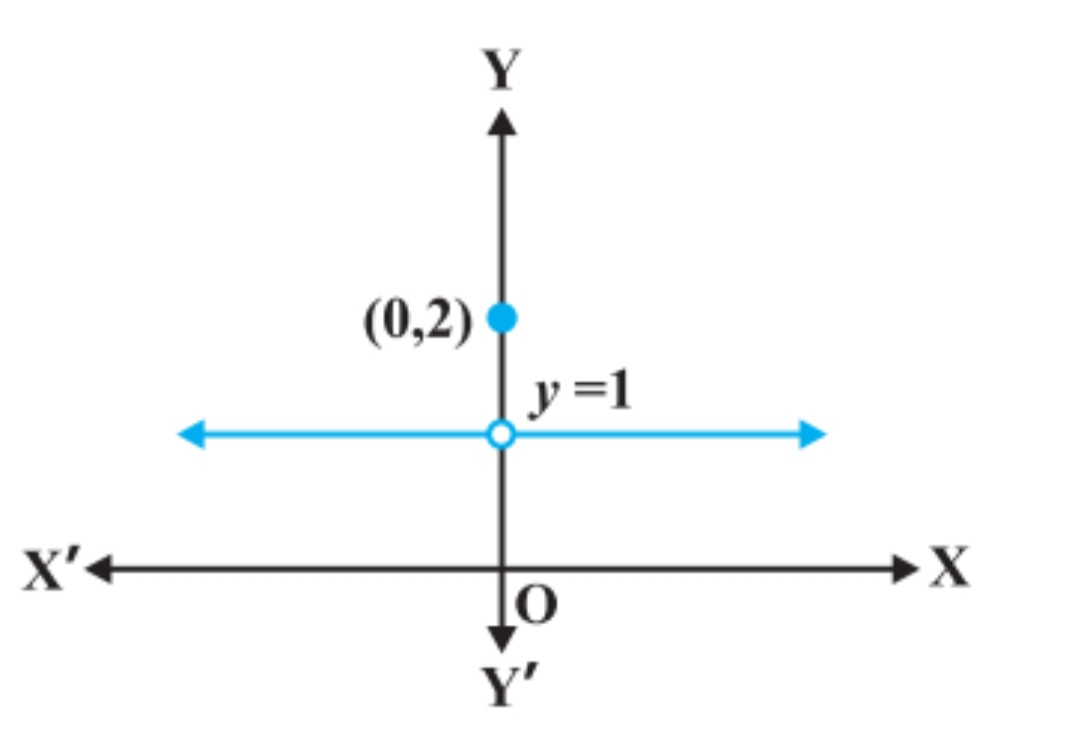
\includegraphics[ width=1\linewidth]{IMG_20250312_201905.jpg} 
\caption\textbf{5.1 Graph of the function}
\end{wrapfigure}


This function is, of course, defined at every point of the real line. The graph of this function is given in Figure 5.1. One can deduce from the graph that the value of the function at nearby points on the x-axis remains close to each other except at \( x = 0 \). At points near and to the left of 0, such as \(-0.1, -0.01, -0.001\), the value of the function is 1. At points near and to the right of 0, such as \(0.1, 0.01, 0.001\), the value of the function is 2.
\vspace{5cm}
Using the language of left and right-hand limits, we may say that the left-hand limit (respectively, right-hand limit) of \( f \) at \( 0 \) is 1 (respectively, 2). 

In particular, the left and right hand limits do not coincide. We also observe that the value of the function at \( x = 0 \) coincides with the left-hand limit. Note that when we try to draw the graph, we cannot draw it in one stroke, i.e., without lifting the pen from the plane of the paper. We cannot draw the graph of this function in one continuous stroke. In fact, we need to lift the pen when we come to 0 from the left. This is one instance of a function being not continuous at \( x = 0 \).

Now, consider the function defined as follows:

\[
f(x) =
\begin{cases}
1, & \text{if } x \neq 0 \\
2, & \text{if } x = 0
\end{cases}
\]

\begin{wrapfigure}{r}{0.4\textwidth}
\centering
\vspace{-2mm}
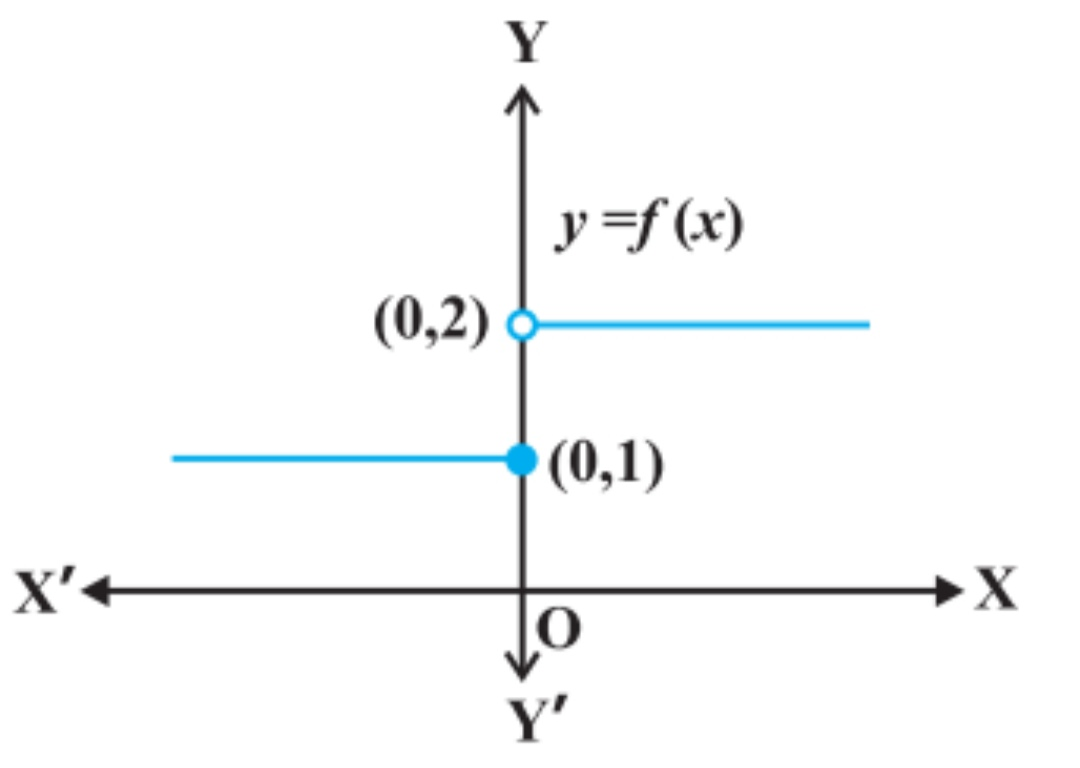
\includegraphics[ width=1\linewidth]{IMG_20250312_185848.jpg} 
\caption\textbf{5.1 Graph of the function}
\end{wrapfigure}

   \hspace{1cm} This function is also defined at every point. The left and right hand limits at \( x = 0 \) are both equal to 1. However, the value of the function at \( x = 0 \) equals 2, which does not coincide with the common value of the left and right hand limits.    

\hspace{1cm} 
Again, we note that we cannot draw the graph of the function without lifting the pen. This is yet another instance of a function being not continuous at \( x = 0 \).

\hspace{1cm} 
Naively, one might say that a function is continuous at a fixed point if we can draw the graph of the function around that point without lifting the pen from the plane of the paper. However, 

\hspace{1cm} Mathematically, the concept of continuity can be phrased more precisely as follows:

\vspace{2cm}

    \textbf{\textcolor{blue}{Definition 1}} Suppose \( f \) is a real function on a subset of the real numbers, and let \( c \) be a point in the domain of \( f \). Then \( f \) is continuous at \( c \) if
    \[
    \lim_{x \to c} f(x) = f(c)
    \]

More elaborately, if the left-hand limit, right-hand limit, and the value of the function at \( x = c \) exist and are equal to each other, then \( f \) is said to be continuous at \( x = c \). Recall that if the right-hand and left-hand limits at \( x = c \) coincide, we say that the common value is the limit of the function at \( x = c \). 

/vspace{2mm}
Hence, we may also rephrase the definition of continuity as follows: a function \( f \) is continuous at \( x = c \) if:

\end{document}
